\section{Neural Networks}
\textcolor{blue}{Explain the use for this section.}\\
\noindent Neural networks are machine learning algorithms inspired by research on the structure and inner workings of brains. \textcolor{red}{[Insert quote (Rosenblatt?)]} Though in the beginning \gls{nns} were not used in computer sciences due to computational limitations \textcolor{red}{[Citation]} they are now a major source of innovation across multiple disciplines. Their capability of pattern recognition and classification has already been successfully applied to a wide range of problems not only in commercial applications but also many scientific fields. \textcolor{red}{[Quote a few scientific usecases here. Of course using the one for gw but also other disciplines.]} Major use cases in the realm of gravitational wave analysis have been classification of glitches in the strain data of \gls{gw}-detectors \textcolor{red}{[Citation]} and classification of strain data containing a \gls{gw} versus pure noise \textcolor{red}{[Citation]}. \textcolor{red}{A few more notable examples include [list of citations].}\\
In this section the basic principles of \gls{nns} will be introduced and notation will be set. The concept of backpropagation will be introduced \textcolor{red}{and extended to a special and for this work important kind of \gls{nn}. (maybe use the term ''convolution'' here already?)} It will be shown that learning in \gls{nns} is simply a mathematical minimization of errors that can largely be understood analytically.\medskip\\
Large portions of this section are inspired and guided by \cite{deep_learning_beginning, deep_learning_book}.

\begin{comment}
Neural networks have become a new and major player in data sciences over the past few years. They have proven to be very good at classification and interpolation. \textcolor{red}{[Insert ref]} Therefore and due to their computational efficiency they seem to be a compelling option even for scientific use cases and have been successfully applied to the classification and basic parameter estimation of \gls{gw}-data.\\
This sections aims to convey the basics of neural networks and the layers that are being utilized in this work. After having read this section it should be clear that neural networks are simply a mathematical model and that there is no magic involved. \textcolor{red}{(Maybe this is too prosa-like and/or should be put into the introduction)}
\end{comment}

\subsection{Neurons, Layers and Networks}\label{sec:basics_neuron_network}
\textcolor{blue}{What is the general concept of a neural network? How does it work? How does backpropagation work? How can one replicate logic gates? (cite online book)}\\
\noindent The basic building block of a \gls{nn} is - as the name suggests - a \emph{neuron}. This neuron is a function mapping inputs to a single output.\\
In general there are two different kinds of inputs to the neuron. Those that are specific to the neuron itself and those that the neuron receives as an outside stimulus. We write the neuron as
\begin{equation}\label{def:neuron}
n: \R^k\times\R\times\R^k\to\R ;\ \ \ (\vec{w}, b, \vec{x})\mapsto n(\vec{w}, b, \vec{x})\coloneqq a(\vec{w}\cdot\vec{x}+b),
\end{equation}
where $\vec{w}$ are called weights, $b$ is a bias value, $\vec{x}$ is the outside stimulus and $a$ is a function known as the \emph{activation function}\textcolor{red}{ (change this to not be emphasized if it is not used for the first time here)}. The weights and biases are what is tweaked to control the behavior of the neuron, whereas the outside stimulus is not controllable in that sense. A usual depiction of a neuron and its structure is shown in \autoref{fig:neuron}.\\
The activation function is a usually nonlinear scalar function
\begin{equation}\label{def:activation_function}
a:\ \R\to\R
\end{equation}
determining the scale of the output of the neuron. The importance of this activation function and its nonlinearity will be touched upon a little later.\\
To understand the role of each part of the neuron, consider the following activation function:
\begin{equation}\label{def:step_activation}
a(y) = 
\begin{cases}
	1,& y> 0\\
	0,& y\leq 0
\end{cases}.
\end{equation}
With this activation function, the neuron will only send out a signal (or ''fire'') if the input $y$ is greater than 0. Therefore, in order for the neuron to fire, the weighted sum of the inputs $\vec{w}\cdot\vec{x}$ has to be larger than the negative bias $b$. This means that the weights and biases control the behavior of the neuron and can be optimized to get a specific output.\\
The effects of changing the weights makes individual inputs more or less important. The closer a weight $w_i$ is to zero, the less impact the corresponding input value $x_i$ will have. Choosing a negative weight $w_i$ results in the corresponding input $x_i$ being inverted, i.e. the smaller the value of $x_i$ the more likely the neuron is to activate and vice versa.\\
Changing the bias to a more negative value will result in the neuron having fewer inputs it will fire upon, i.e. the neuron is more difficult to activate. The opposite is true for larger bias values. So increasing it will result in the neuron firing for a larger set of inputs.\\
As an example consider a neuron with activation function \eqref{def:step_activation}, weights $\vec{w}={(w_1, w_2)}^T=(1, 1)$, bias $b=-1.5$ and inputs $(x_1,x_2)\in{\{0,1\}}^2$. Choosing the weights and biases in this way results in the outputs shown in \autoref{tab:and_neuron}. This goes to show that neurons can replicate the behavior of an ''and''-gate. Other logical gates can be replicated by choosing the weights and biases in a similar fashion.
\begin{table}
\begin{center}
\begin{tabular}{c c|c}
$x_1$ & $x_2$ & $a(\vec{w}\cdot\vec{x}+b)$\\
\hline
$0$ & $0$ & $0$\\
$0$ & $1$ & $0$\\
$1$ & $0$ & $0$\\
$1$ & $1$ & $1$\\
\end{tabular}
\caption[''OR''-neuron activations]{Neuron activation with activation function \eqref{def:step_activation}, weights $\vec{w}={(w_1, w_2)}^T=(1, 1)$, bias $b=-1.5$ and inputs $(x_1,x_2)\in{\{0,1\}}^2$. Choosing the weights and biases in this way replicates an ''and''-gate.}\label{tab:and_neuron}
\end{center}
\end{table}

\begin{figure}
\centering
\begin{tikzpicture}[
neuron/.style={circle, draw=black, very thick, minimum size=1.5cm},
dot/.style={circle, draw=black, fill=black, minimum size=0.1cm, inner sep=0pt},
VLineVertex/.style={circle, draw=black, minimum size=0cm, inner sep=0pt},
]

\node[neuron] (neuron) {$a, \vec{w}, b$};
\node (x2) [left=2cm of neuron] {$x_2$};
\node (x1) [above=0.5cm of x2] {$x_1$};
\node (x3) [below=0.5cm of x2] {$x_3$};
\node (out) [right=2cm of neuron] {$a(\vec{w}\cdot\vec{x}+b)$};

\draw (x1.east) -- (neuron.west);
\draw (x2.east) -- (neuron.west);
\draw (x3.east) -- (neuron.west);
\draw [->] (neuron.east) -- (out.west);

\end{tikzpicture}
\caption[Neuron]{Depiction of a neuron with inputs $\vec{x}={(x_1, x_2, x_3)}^T$, weights $\vec{w}$, bias $b$ and activation function $a$.}\label{fig:neuron}
\end{figure}

\medskip
\textcolor{blue}{Use the introduction of the and-neuron from above to introduce the concept of networks in a familiar way. Having logic gates enables us to build more complex structures, such as full adders and hence we can, in principle, calculate any function a computer can calculate. Only afterwards introduce layers as a way of structuring and formalizing networks.}\\
\noindent Since all basic logic gates can be replicated by a neuron, it is a straight forward idea to connect them into more complicated structures, like a full-adder (see \autoref{app:Full_adder}). These structures are than called neural networks, as they are a network of neurons. The example of the full-adder demonstrates the principle of a \gls{nn} perfectly. Its premise is to connect multiple simple functions, the neurons, to form a network, that can solve tasks the individual building blocks can't.\\
In other words, a network aims to calculate some general function by connecting multiple easier functions together. This highlights the importance of the activation function, as it introduces nonlinearities into the network. Without these a neural network would not be able to approximate a nonlinear function such as the XOR-Gate used in \autoref{app:Full_adder} (section 6.1 in \cite{deep_learning_book}), which caused the loss of interest in \gls{nns} around 1940 (section 6.6 in \cite{deep_learning_book}).\medskip\\
Since \gls{nns} are the main subject of \autoref{sec:backpropagation} and since it will be a bit more mathematical, some notation and nomenclature is introduced to structure the networks.\\
Specifically each network can be structured into multiple layers. Each layer consists of one or multiple neurons and each neuron has inputs only from previous layers. Formally we write
\begin{equation}
\mathcal{L}:\R^{k\times l}\times\R^l\times\R^k\to\R^l;\ (W, \vec{b}, \vec{x})\mapsto\mathcal{L}(W,\vec{b},\vec{x})\coloneqq
\begin{pmatrix}
n_1\lr{{(W_1)}^T,b_1,\vec{x}}\\
\vdots\\
n_l\lr{{(W_l)}^T,b_l,\vec{x}}
\end{pmatrix},
\end{equation}
where $n_i$ is neuron $i$ on the layer and $W_i$ is the $i$-th row of a $k\times l$-matrix. In principle this definition can be extended to tensors of arbitrary dimensions. This would however only complicate the upcoming sections notationally and the principle should be clear from this minimal case, as dot products, sums and other operations have their according counterparts in tensor calculus. As a further step of formal simplification we will assume that all neurons $n_i$ share the same activation function $a$. This does not limit the ability of networks that can be written down, since if two neurons have different activation functions, they can be viewed as two different layers connected to the same previous layer. Their output will than be merged afterwards (see \autoref{fig:diff_activation_functions_layer}).\\
\begin{figure}
\centering
\begin{tikzpicture}[
neuron/.style={circle, draw=black, very thick, minimum size=1.4cm},
dot/.style={circle, draw=black, fill=black, minimum size=0.1cm, inner sep=0pt},
VLineVertex/.style={circle, draw=black, minimum size=0cm, inner sep=0pt},
layer/.style={rectangle, draw=black, very thick, minimum height=1.7cm, minimum width=1cm}
]

\node[layer] (in1) {$\mathcal{L}_\text{in}$};
\node[layer] (n1n2) [right=1cm of in1] {$\oset[4ex]{n_1}{n_2}$};

\node[layer] (out1) [right=1cm of n1n2] {$\mathcal{L}_\text{out}$};
\node (lmid) [above=0.2cm of n1n2] {$\mathcal{L}_\text{mid}$};

\node (arrow_start) [right=0.5cm of out1] {};
\node (arrow_end) [right=0.75cm of arrow_start] {};

\node[layer] (in2) [right=0.5cm of arrow_end] {$\mathcal{L}_\text{in}$};
\node (midpoint) [right=1.5cm of in2] {};
\node[layer] (ln1) [above=0.2cm of midpoint] {$\mathcal{L}_{n_1}$};
\node[layer] (ln2) [below=0.2cm of midpoint] {$\mathcal{L}_{n_2}$};
\node[layer] (out2) [right=1.5cm of midpoint] {$\mathcal{L}_\text{out}$};

%Connections part1
\draw (in1.east) -- (n1n2.west);
\draw (n1n2.east) -- (out1.west);

%Arrow
\draw[->] (arrow_start) -- (arrow_end);

%Connections part2
\draw (in2.east) -- (ln1.west);
\draw (in2.east) -- (ln2.west);
\draw (ln1.east) -- (out2.west);
\draw (ln2.east) -- (out2.west);
\end{tikzpicture}
\caption[Splitting different actvation functions into seperate layers]{Depiction of how a layer ($\mathcal{L}_\text{mid}$) consisting of neurons with different activation functions ($n_1$ and $n_2$) can be split into two separate layers ($\mathcal{L}_{n_1}$ and $\mathcal{L}_{n_2}$).}\label{fig:diff_activation_functions_layer}
\end{figure}

\noindent With this simplification one can write a layer simply as
\begin{equation}
\mathcal{L}(W,\vec{b},\vec{x})=a(W\cdot\vec{x}+\vec{b}),
\end{equation}
where it is understood, that the activation function $a$ acts component wise on the resulting $l$-dimensional vector.\\
In this fashion a network consisting of a chain of layers $\mathcal{L}_\text{in}$, $\mathcal{L}_\text{mid}$, $\mathcal{L}_\text{out}$ can be written as
\begin{align}
\mathcal{N} & \lr{W^\text{in}, \vec{b}^\text{in}, W^\text{mid}, \vec{b}^\text{mid}, W^\text{out}, \vec{b}^\text{out}, \vec{x}}\nonumber\\
\phantom{\mathcal{N}} & \coloneqq\mathcal{L}_\text{out}\lr{W^\text{out}, \vec{b}^\text{out}, \mathcal{L}_\text{mid}\lr{W^\text{mid}, \vec{b}^\text{mid}, \mathcal{L}_\text{in}\lr{W^\text{in}, \vec{b}^\text{in}, \vec{x}}}}\nonumber\\
\phantom{\mathcal{N}} & = a_\text{out}\lr{\vec{b}^\text{out}+W^\text{out}\cdot a^\text{mid}\lr{\vec{b}^\text{mid}+W_\text{mid}\cdot a_\text{in}\lr{\vec{b}^\text{in}+W_\text{in}\cdot \vec{x}}}}.
\end{align}
Hence a network can be understood as a set of nested functions.\\
An important point with the definitions above is that the layers get their input only from their preceding layers. Especially no loops are allowed, i.e. getting input from some subsequent layer is not permitted. A network of the first kind is called a \emph{feed forward neural network} (\gls{ffn}), as the input to the network is propagated from front to back, layer by layer and each layer gets invoked only once. There are also other architectures called \emph{recurrent neural networks} (\gls{rnn}), which allow for loops and work by propagating the activations in discrete time steps. These kinds of networks are in principle closer to the inner workings of the human brain, but in practice show worst performance and are therefore not used or discussed further in this work. \textcolor{red}{[Citations], maybe also mention that RNNs have shown good performance in time series data (which we are working with) but other studies (paper Frank sent around) have shown that TCN also do the job}\\
A \gls{ffn} can in general be grouped into three different parts called the input-, output- and hidden layer/layers. The role of the input- and output-layers is self explanatory; they are the layers where data is fed into the network or where data is read out. Therefore their shape is determined by the data the network is being fed and the expected return. The hidden-layers on the contrary are called ''hidden'', as their shape and size is not defined by the data. Furthermore the hidden layers do not see the input or labels directly, which means that the network itself has to ''decide'' on how to use them (page 165 in \cite{deep_learning_book}). \autoref{fig:hidden_layer} shows an example of a simple network with a single hidden layer. In principle there could be any number of hidden layers with different sizes. In this example the input is n-dimensional and the output 2-dimensional. If the input was changed to be (n-1)-dimensional, the same hidden-layer could be used, as its size does not depend on the data or output. Therefore, when designing a network architecture, one designs the shape and functionality of the hidden layers. How well it performs is mainly governed by theses layers. Two networks with different hidden layers are also called different architectures. The architecture of a neural network hence describes how all layers of the network behave and are connected. \textcolor{red}{[Can I find citation for these last statements?]}\\
A \gls{nn} is called \emph{deep}, if it has multiple hidden layers. The depth of a network analogously is number of layers at the longest path to an output layer. \textcolor{red}{[Citation]}
\begin{figure}
\centering
\begin{tikzpicture}[
neuron/.style={circle, draw=black, very thick, minimum size=1cm, transform shape},
dot/.style={circle, draw=black, fill=black, minimum size=0.1cm, inner sep=0pt, transform shape},
note/.style={circle, draw=black, minimum size=0pt, inner sep=0pt, transform shape},
]

%Input Layer neurons
\node[neuron] (inp_1) {};
\node[neuron] (inp_2) [below=0.3cm of inp_1] {};
\node[dot] (inp_v_1) [below=0.3cm of inp_2] {};
\node[dot] (inp_v_2) [below=0.15cm of inp_v_1] {};
\node[dot] (inp_v_3) [below=0.15cm of inp_v_2] {};
\node[neuron] (inp_3) [below=0.3cm of inp_v_3] {};
\node[neuron] (inp_4) [below=0.3cm of inp_3] {};
\node (inp_label) [above=0.3cm of inp_1] {Input Layer};

%Hidden Layer neurons
\node[dot] (hid_v_2) [right=3cm of inp_v_2] {};
\node[dot] (hid_v_1) [above=0.15cm of hid_v_2] {};
\node[dot] (hid_v_3) [below=0.15cm of hid_v_2] {};
\node[neuron] (hid_2) [above=0.3cm of hid_v_1] {};
\node[neuron] (hid_1) [above=0.3cm of hid_2] {};
\node (hid_label) [above=0.3cm of hid_1] {Hidden Layer};
\node[neuron] (hid_3) [below=0.3cm of hid_v_3] {};
\node[neuron] (hid_4) [below=0.3cm of hid_3] {};

%Output Layer neurons
\node[note] (out_mid) [right=3cm of hid_v_2] {};
\node[neuron] (out_1) [above=0.15cm of out_mid] {};
\node[neuron] (out_2) [below=0.15cm of out_mid] {};
\node (out_label) [above=3.25cm of out_mid] {Output Layer};

%Inputs
\node (x1) [left=1cm of inp_1] {$x_1$};
\node (x2) [left=1cm of inp_2] {$x_2$};
\node (x3) [left=1cm of inp_3] {$x_{n-1}$};
\node (x4) [left=1cm of inp_4] {$x_n$};

%Outputs
\node (o1) [right=1cm of out_1] {Output 1};
\node (o2) [right=1cm of out_2] {Output 2};

%Connections Input Layer - Hidden Layer
\draw (inp_1.east) -- (hid_1.west);
\draw (inp_1.east) -- (hid_2.west);
\draw (inp_1.east) -- (hid_3.west);
\draw (inp_1.east) -- (hid_4.west);

\draw (inp_2.east) -- (hid_1.west);
\draw (inp_2.east) -- (hid_2.west);
\draw (inp_2.east) -- (hid_3.west);
\draw (inp_2.east) -- (hid_4.west);

\draw (inp_3.east) -- (hid_1.west);
\draw (inp_3.east) -- (hid_2.west);
\draw (inp_3.east) -- (hid_3.west);
\draw (inp_3.east) -- (hid_4.west);

\draw (inp_4.east) -- (hid_1.west);
\draw (inp_4.east) -- (hid_2.west);
\draw (inp_4.east) -- (hid_3.west);
\draw (inp_4.east) -- (hid_4.west);

%Connections Hidden Layer - Output Layer
\draw (hid_1.east) -- (out_1.west);
\draw (hid_1.east) -- (out_2.west);

\draw (hid_2.east) -- (out_1.west);
\draw (hid_2.east) -- (out_2.west);

\draw (hid_3.east) -- (out_1.west);
\draw (hid_3.east) -- (out_2.west);

\draw (hid_4.east) -- (out_1.west);
\draw (hid_4.east) -- (out_2.west);

\draw[->] (x1) -- (inp_1.west);
\draw[->] (x2) -- (inp_2.west);
\draw[->] (x3) -- (inp_3.west);
\draw[->] (x4) -- (inp_4.west);

\draw[->] (out_1.east) -- (o1);
\draw[->] (out_2.east) -- (o2);
\end{tikzpicture}
\caption[Simple neural network]{A depiction of a simple network with a single input-, hidden- and output-layer. The input-data is a n-dimensional vector ${(x_1, \dotsc, x_n)}^T$ and the output is a 2-dimensional vector. In this picture it looks like the hidden layer has the same number of neurons as the input layer. This does not necessarily have to be the case. Lines between two neurons indicate, that the output of the left neuron serves as weighted input for the right one.}\label{fig:hidden_layer}
\end{figure}

\subsection{Backpropagation}\label{sec:backpropagation}
\textcolor{red}{The beginning of this section feels very wordy and repetitive. Break it down!}\\
In \autoref{sec:basics_neuron_network} the basics of a \gls{nn} where discussed and the example of a network replicating a binary full-adder showed the potential of these networks, when the weights and biases are chosen correctly. The example actually proofs that a sufficiently complicated network can - in principle - calculate any function a computer can, as a computer is just a combination of logic gates, especially binary full-adders.\footnote{There is an even stronger statement called the universal approximation theorem, which states that any Borel measurable function on a finite-dimensional space can be approximated to any degree with a \gls{nn} with at least one single hidden layer of sufficient size. (p. 194 \cite{deep_learning_book})}\cite{deep_learning_beginning}\\
The question therefore is how to choose the weights in a network for it to approximate some function optimally. For the binary full-adder the weights and biases were chosen by hand, as the problem the network was trying to solve was rather simple. A more general approach however would be beneficial, as not all problems are this simple. Therefore the goal is to design some network and let it learn/optimize the weights and biases such that the error between the actual function and the estimate of the network is minimal.\\
To do this, some known and labeled data is necessary, in order for the network being able to compare its output to some ground truth and adjust its weights and biases to minimize some error function. This way of optimizing the weights and biases is called \emph{training}. The data used during training is hence called training data or training set. To be a bit more specific, the analyzed data in this work is some time series. The output of this analysis will be some scalar number; the \gls{snr}. Therefore the network receives some data as input, of which the true \gls{snr}-value is known. This true value will be called \emph{label}\footnote{For regression problems this value is often also called target value. We will however stick to calling it the label for our training data.} from here on out. The network will produce some value from this input data and compare it to what \gls{snr} was provided as label. From there it will try to optimize the weights and biases to best fit the function that maps $\text{data}\to\text{\gls{snr}}$. This process of optimizing the weights and biases in the way described below is enabled by a process called backpropagation, as the error propagates from the last to the first layer. The meaning of this will become clearer in the upcoming paragraphs.\\
So far only the abstract term ''error'' was used. This error, in machine learning language, is called the \emph{loss function} and in general is defined by
\begin{equation}\label{def:general_loss}
L:\R^{l\times k}\times\R^{l\times k}\to\R;\ (y_\text{net}, y_\text{label})\mapsto L(y_\text{net}, y_\text{label}),
\end{equation}
where $l$ is the number of training samples used to estimate the error and $k$ is the dimension of the network output.\\
When doing a regressive fit, one of the standard error functions is the \emph{mean squared error} (\gls{mse}), which is the loss function mainly used in this work and that is defined by
\begin{equation}\label{def:loss_mean_squared_error}
L:\R^{l\times k}\times\R^{l\times k}\to\R;\ (y_\text{net}, y_\text{label})\mapsto L(y_\text{net}, y_\text{label})\coloneqq\frac{1}{l}\sum_{i=1}^l{(\vec{y}_{\text{net},i}-\vec{y}_{\text{label},i})}^2.
\end{equation}
A more thorough discussion and justification for using \gls{mse} as loss can be found in section 5.5 and 6.2.1.1 of \cite{deep_learning_book}.\\
To minimize this loss, the weights and biases of the different layers are changed, usually using an algorithm called \emph{gradient decent}. It works by calculating the gradient of some layer with respect to its weights and biases and taking a step in the opposite direction. For notational simplicity we'll denote the weights and biases of a network by $\theta$ and call them collectively parameters. It is understood that $\theta=\lr{W^{1},b^1, W^2, b^2, \cdots}$. Gradient decent is than given by
\begin{equation}\label{def:gradient_decent}
\theta '=\theta - \epsilon\ \nabla_\theta L\lr{y_\text{net}(\theta), y_\text{label}},
\end{equation}
where $\epsilon$ is called learning rate and controls how large of a step is taken on each iteration.\\
This formula assumes, that all samples from the training set are used to calculate the gradient. In practice this would be too computationally costly. Therefore the training set is split into multiple parts, called mini-batches. A step of the gradient decent is than made using only the samples from one mini-batch. This alteration of gradient decent goes by the name of \emph{stochastic gradient decent} (\gls{sgd}). The larger the mini-batch, the more accurate the estimate of the gradient and therefore the fewer steps are needed to get to lower values of the loss. Each step however takes longer to calculate. This means one has to balance the benefits and drawbacks of the mini-batch size.\medskip\\
The real work of training a network now lies in calculating the gradient $\nabla_\theta L\lr{y_\text{net}(\theta), y_\text{label}}$, which is a challenge, as $\theta$ usually consists of at least a few hundred thousand weights and biases. The algorithm, that is used to calculate this gradient, is called backpropagation or simply backprop and is mostly a iterative application of the chain rule.\\
For simplicity assume we have a network $\mathcal{N}\lr{\theta, \vec{x}}$ consisting of $n$ consecutive layers $\mathcal{L}^1,\cdots,\mathcal{L}^n$ with weights $W^1,\cdots,W^n$, biases $\vec{b}^1,\cdots,\vec{b}^n$ and activation functions $a_1,\cdots, a_n$. The network will be trained by minimizing the loss given in \eqref{def:loss_mean_squared_error}. Calculating the gradient $\nabla_\theta L\lr{y_\text{net}(\theta), y_\text{label}}$ requires to calculate $\nabla_{W^1}L, \cdots,\nabla_{W^n}L$ and $\nabla_{\vec{b}^1}L,\cdots,\nabla_{\vec{b}^n}L$, where
\begin{equation}\label{def:matrix_gradient}
\nabla_{W^i}L\coloneqq
\begin{pmatrix}
	\partial_{W^i_{11}}L & \cdots & \partial_{W^i_{1l}}L\\
	\vdots & \ddots & \vdots\\
	\partial_{W^i_{k1}}L & \cdots & \partial_{W^i_{kl}}L
\end{pmatrix},
\end{equation}
for $W^i\in \R^{k\times l}$ and
\begin{equation}\label{def:vector_gradient}
\nabla_{\vec{b}^i}L\coloneqq
\begin{pmatrix}
	\partial_{b^i_1}L\\
	\vdots\\
	\partial_{b^i_k}L
\end{pmatrix},
\end{equation}
for $\vec{b}^i\in\R^k$.\\
To calculate $\partial_{W^i_{jk}}L$ and $\partial_{b^i_j}L$, define
\begin{align}\label{def:backprop_z}
z^n & \coloneqq\vec{b}^n+W^n\cdot a_{n-1}\lr{z^{n-1}}\nonumber\\
z^1 & \coloneqq\vec{b}^1+W^1\cdot\vec{x},
\end{align}
such that
\begin{equation}
\mathcal{N}\lr{\theta,\vec{x}}=a_n\lr{z_n}.
\end{equation}
To save another index, we will assume a mini-batch size of 1. For a larger mini-batch size one simply has to average over the individual gradients, as sums and derivatives commute.\\
With this in mind, the loss is given by
\begin{equation}
L\lr{y_\text{net}, y_\text{label}}=L\lr{\mathcal{N}\lr{\theta,\vec{x}}, y_\text{label}}=L\lr{a_n\lr{z_n}, y_\text{label}}=\lr{a_n\lr{z_n}- \vec{y}_\text{label}}^2.
\end{equation}
To start off derive this loss by the parameter $\theta_j$
\begin{equation}
\partial_{\theta_j}\lr{a_n\lr{z_n}- \vec{y}_\text{label}}^2=\lr{\partial_{\theta_j}a_n\lr{z_n}}\lr{2\lr{a_n\lr{z_n}- \vec{y}_\text{label}}}
\end{equation}
From there calculate $\partial_{\theta_j}a_n\lr{z_n}$, remembering, that $a_n$ and $z_n$ are both vectors.
\begin{align}\label{def:start_backprop}
\partial_{\theta_j}a_n\lr{z_n} & = \partial_{\theta_j}\sum_i a_n^i\lr{z_{n,1}\lr{\theta_j},\dotsc, z_{n,k}\lr{\theta_j}} \vec{e}_i\nonumber\\
& = \sum_i \sum_{m=1}^k \lr{\partial_{\theta_j}z_{n, m}\lr{\theta_j}}\lr{\partial_{z_{n, m}} a_n^i\lr{z_{n,1}\lr{\theta_j},\dotsc, z_{n,k}\lr{\theta_j}}} \vec{e}_i\nonumber\\
& = \sum_i \lr{\lr{\partial_{\theta_j}z_n}\cdot \lr{\nabla_{z_n} a_n^i}}\vec{e}_i
\end{align}
Since all activation functions $a_n^i$ on a layer are the same, the gradient $\lr{\nabla_{z_n} a_n^i}$ simplifies to $\partial_z \restr{a(z)}{z=z_{n,i}}$. With this one gets
\begin{equation}\label{def:start_backprop_simple}
\partial_{\theta_j}a_n\lr{z_n} = \lr{\partial_{\theta_j} z_n} \odot \partial_z \restr{a_n(z)}{z=z_n},
\end{equation}
where $\odot$ denotes the Hadamard product.
The final step to understanding backpropagation is to evaluate $\partial_{\theta_j}z_n$. For now assume that $\theta_j$ is some weight on a layer that is not the last layer.
\begin{align}\label{def:backprop_recurs_1}
\partial_{\theta_j}z_n & = \partial_{\theta_j}\lr{\vec{b}^n+W^n\cdot a_{n-1}\lr{z_{n-1}}}\nonumber\\
& = \partial_{\theta_j}\lr{W^n\cdot a_{n-1}\lr{z_{n-1}}}\nonumber\\
& = W^n\cdot\partial_{\theta_j}a_{n-1}\lr{z_{n-1}}
\end{align}
Inserting \eqref{def:backprop_recurs_1} into \eqref{def:start_backprop_simple} yields the recursive relation
\begin{equation}\label{def:backprop_recursive_relation}
\partial_{\theta_j}a_n\lr{z_n} = \lr{W^n\cdot\partial_{\theta_j}a_{n-1}\lr{z_{n-1}}}\odot\partial_z \restr{a_n(z)}{z=z_n}.
\end{equation}
The recursion stops, when it reaches the layer the weight $\theta_j$ is located on and evaluates to (assuming $\theta_j$ is part of layer $k$)
\begin{equation}\label{def:recursion_stop_weight}
\partial_{\theta_j}a_k\lr{z_k}=\lr{\partial_{\theta_j}W^k}\cdot a_{k-1}\lr{z_{k-1}}.
\end{equation}
The derivative can also be expressed in an analytical form, by utilizing, that the Hadamard product is commutative and can be expressed in terms of matrix multiplications. To do so define
\begin{equation}
\left[\Sigma\lr{\vec{x}}\right]_{ij}=
\begin{cases}
	x_i,& i = j\\
	0,& \text{otherwise}
\end{cases}.
\end{equation}
With this definition equation \eqref{def:backprop_recursive_relation} can be written as
\begin{equation}
\partial_{\theta_j}a_n\lr{z_n} = \Sigma\lr{\partial_z \restr{a_n(z)}{z=z_n}}\cdot W^n\cdot\partial_{\theta_j}a_{n-1}\lr{z_{n-1}}
\end{equation}
and the recursion can be solved to yield
\begin{equation}\label{def:backprop_analytical_weight}
\partial_{\theta_j}a_n\lr{z_n} = \left[\prod_{l=0}^{n-k+1}\Sigma\lr{\restr{\partial_z a_{n-l}\lr{z}}{z=z_{n-l}}}\cdot W^{n-l}\right]\cdot \Sigma\lr{\restr{\partial_z a_k\lr{z}}{z=z_k}}\cdot\lr{\partial_{\theta_j}W^k}a_{k-1}\lr{z_{k-1}}.
\end{equation}
\textcolor{red}{If there is time, check the equations below, as I did not thoroughly recompute them.}\\
The same computation can be done if $\theta_j$ is a bias instead of a weight. When this computation is done, equation \eqref{def:backprop_recursive_relation} still holds, but the stopping condition \eqref{def:recursion_stop_weight} is simplified to
\begin{equation}
\partial_{\theta_j}a_k\lr{z_k}=\partial_{\theta_j}\vec{b}^k.
\end{equation}
From this the analytic form can be computed to be
\begin{equation}\label{def:backprop_analytical_bias}
\partial_{\theta_j}a_n\lr{z_n} = \left[\prod_{l=0}^{n-k+1}\Sigma\lr{\restr{\partial_z a_{n-l}\lr{z}}{z=z_{n-l}}}\cdot W^{n-l}\right]\cdot \Sigma\lr{\restr{\partial_z a_k\lr{z}}{z=z_k}}\cdot\partial_{\theta_j}\vec{b}^k.
\end{equation}
The recursive formula \eqref{def:backprop_recursive_relation} now justifies the term ''backpropagation''. When a sample is evaluated, it is passed from layer to layer starting at the front. Therefore this is called a \emph{forward pass}. The output the network gives for a single forward pass will probably differ from the label and hence has an error (quantified by the loss function). This error is used to calculate the gradient and adjusts the parameters of the network. The way this is done is given by \eqref{def:backprop_recursive_relation}. It starts at the last layer and propagates back through the network until it reaches the layer of the weight that should be adjusted.\\
With these formulae one could in principle calculate the gradient of the loss with respect to all parameters $\theta$ and use this gradient to optimize and train a network. In reality this would still be too slow and computationally costly. Instead each layer (or rather each operation) has a backpropagation method associated to it, that returns the gradient based on a derivative to one of its inputs and the gradient from the previous layer.\\
For clarification, consider an operation that multiplies two matrices $A$ and $B$ and say the gradient calculated by the backpropagation method of the previous layer returned $G$ as its gradient. The backpropagation method for the matrix multiplication now needs to implement the derivative with respect to $A$ and the derivative with respect to $B$. Thus it will return $G\cdot B^T$ when derived by $A$ and $G\cdot A^T$ when derived by $B$. (section 6.5.6 \cite{deep_learning_book})\\
The full backpropagation algorithm than only has to call the backpropagation methods of each layer/operation. (For a more thorough discussion see section 6.5 of \cite{deep_learning_book}.)

\subsection{Training and Terminology}\label{sec:training}
In the previous \autoref{sec:backpropagation} the backpropagation algorithm was introduced as the method used for the network to learn. It used some labeled data to compare its output to and adjust the parameters accordingly. This labeled data was called the training set. In principle the network could be trained over and over again on the same data to further improve the performance of the network. This is done to some extend in practice. An entire pass of the training set is called an \emph{epoch}. In theory, the worst one could fear for is a gradient that vanishes, as the global or a local minimum in the loss is reached.\\
In practice this is true only partially. At some point the network will start ''memorizing'' the samples it has seen in the training set. When a network shows this behavior during training it is called \emph{overfitting}. This is a problem not only known in machine learning but also with regressive fits and has the same reason; too many free parameters. Consider a parabola sampled at $n$ points. If a regressive fit is done, the best choice for the model would be a parabola $f(x)=a x^2+b x + c$ with the three free parameters $a$, $b$ and $c$. If $n\geq 3$ a regressive fit minimizing the \gls{mse} would recover the original parabola that was sampled by the $n$ points. However one could also use a polynomial of degree $m\geq n$ as a model to find a function that runs exactly through all $n$ points and thus minimizes the \gls{mse} to the same value of zero too. (see \autoref{fig:overfitting})\\
There are however two differences between the two cases. The most obvious one is the number of free parameters. The parabola has three parameters, whereas the polynomial of degree $m$ has $m+1$ free parameters. As $m\geq n$ was required, there is at least one parameter that cannot be fixed by the data and is therefore still free. The second difference is the behavior of the \gls{mse} when the fitted model is evaluated on a point, that is not part of the set of points, that was used to generate the fit. For the parabola the \gls{mse} will stay zero, for the polynomial of degree $m$ however the \gls{mse} will most likely be greater than zero, as the true parabola isn't matched. (Compare lower right of \autoref{fig:overfitting}) The first difference explains why overfitting takes place, there are too many parameters that can be varied, the second difference gives a way to detect when overfitting takes place. If the \gls{mse} rises on samples that were not used for the regression, overfitting takes place.\\
The same concept can than be applied to \gls{nns}; if the loss of a network is bigger on different data than that used during training, the network is said to overfit. This second set of samples is called the validation set, as it validates the training. Obviously the data in the validation set must stem from the same underlying procedure, that generated the training set. In the context of this work this means, that the waveforms of the training and validation set must share the same parameter-space.\\
Contrary to overfitting, there is also a phenomenon called \emph{underfitting}. This occurs, when the number of free, i.e. trainable, parameters of a network is too low. It manifests usually in an occasionally lower loss value of the validation set when compared to the training set. To overcome this issue one can simply increase the number of trainable parameters the network has. Increasing the number of trainable parameters is also called increasing the \emph{capacity} of the network.\\
Though underfitting is possible, overfitting is usually a lot more common. There are multiple ways to deal with a network, that overfits during training. The first one would be to reduce the capacity of the network. If that is not possible or worsens the results, the second most easy way is to increase the number of samples in the training set. In the realm of this work, this is a possibility, as we use simulated data, that can be generated on demand. For a lot of other applications however this is not feasible and other means are necessary. One way is to use a technique called regularization, which is explained in \autoref{sec:regularization} and applied to our networks as well. Another one, which will not be discussed in detail here, is data augmentation\footnote{Data augmentation is the process of applying transformations to the input samples, to artificially create more data. The transformation have to act in such a way that the resulting data is similar in its properties to the original data.}. (See section 7.4 of \cite{deep_learning_book})\\
To tune out the generalization error, which is the loss value of the validation set, one adjusts the architecture. If there are multiple different architectures, the best one is chosen by the performance on the validation set. In this way, the validation set is also used to fit the model, as in the end the human who trains the models selects the best performing network. Therefore all given results, that did not occur during training\footnote{An example of a result that comes from training the network would be the loss history.}, come from a third independent set. This set is than called the test set.\medskip\\
A general approach to increase the performance of a network is to increase its depth. This is due to two reasons. First of all it has been shown, that a deep network can separate the underlying function it is trying to learn into piecewise linear regions. The number of these regions is than exponential in the depth of the network. Secondly each layer can be viewed as a filter, that looks for certain features in the data. Having multiple stacked layers will enable the network to learn low level features on early layers and combine them into more difficult features on lower layers. (Section 6.4.1 \cite{deep_learning_book}) This idea will be expanded upon in the following \autoref{sec:cnn}. The depth is not the only parameter of a simple network, that can be scaled to increase performance. A systematic study can be found for instance in \cite{efficient_net}.\\
A common problem, that arises when training very deep \gls{nns} is the vanishing gradient problem; the gradient calculated by \eqref{def:backprop_analytical_weight} or \eqref{def:backprop_analytical_bias} is close to zero on early layers, which results in these layers not changing their weights enough. The reason for this behavior can also be understood from \eqref{def:backprop_analytical_weight} and \eqref{def:backprop_analytical_bias}. If the products satisfy $\left|\partial_z a_i(z)\cdot W^i\right|<1$ the gradient is exponentially diminished by the depth of the network.\\
The opposite can also happen. If $\left|\partial_z a_i(z)\cdot W^i\right|>1$ for most of the layers, the gradient will grow exponentially. This behavior is therefore called the exploding gradient problem. (Chapter 5 \cite{deep_learning_beginning})\\
To overcome these problems, one can simply train for longer periods in the case of the vanishing gradient problem (Chapter 5 \cite{deep_learning_beginning}), use multiple points at which the loss is calculated \cite{inception_module} or adjust the initialization of the weights. Another solution introduced by \cite{residual_connections_invention} are residual connections. These are connections of a layers input to its output. Specifically, the input of the layer is added back onto its output. The idea behind this connection is to make it easier for the network to learn an identity mapping by simply setting the weights of the layer to zero. This showed great improvements and the ability to have very deep networks\cite{residual_connections_invention}.
\begin{figure}
\centering
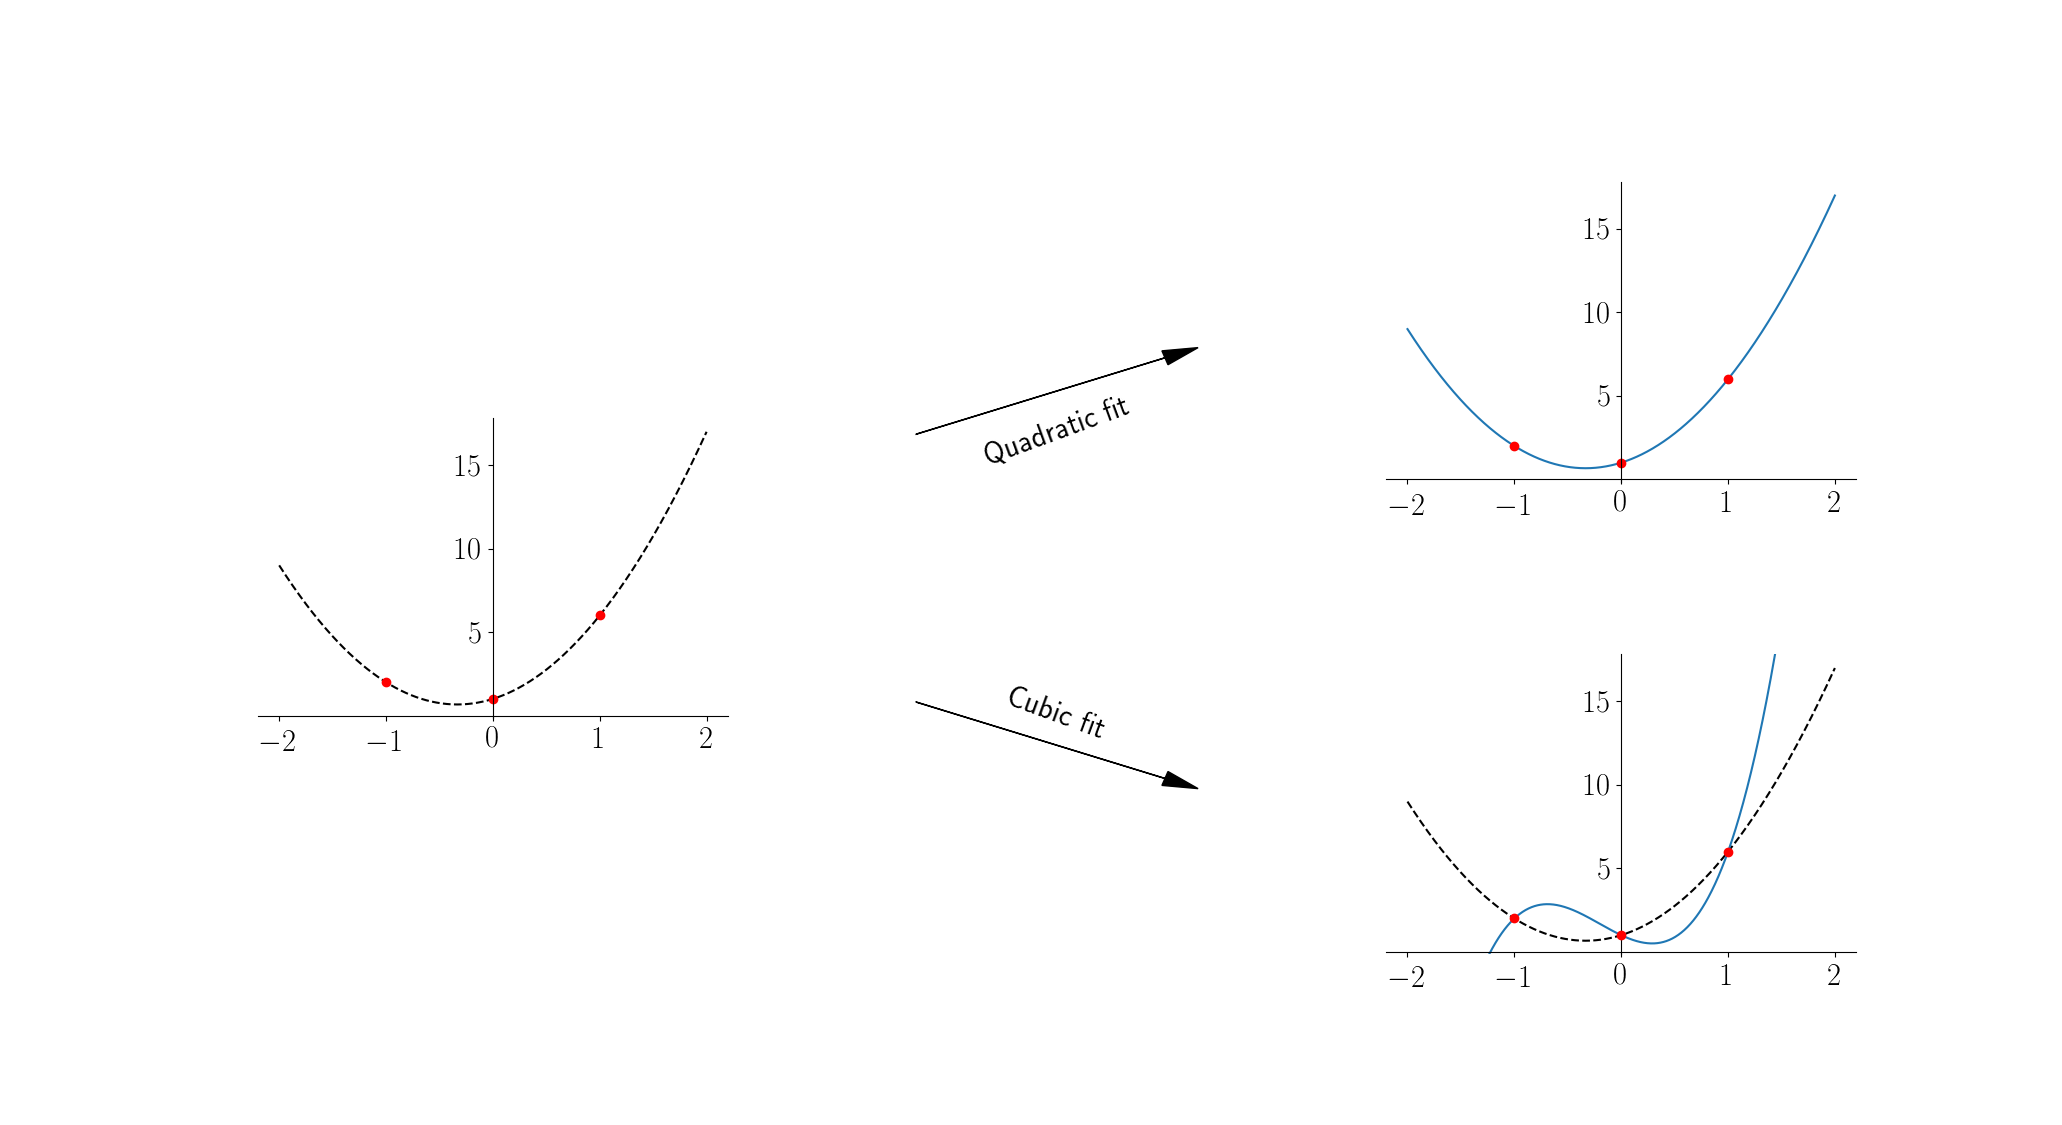
\includegraphics[width=\textwidth]{overfitting.png}
\caption[Overfitting]{Depiction of overfitting in the classical regression. On the left the originally sampled function $f(x)\coloneqq 3x^2 + 2x + 1$ is shown in dashed and black. The red dots are the samples that are being used for the regression on the right. The top right shows the regression, where $g(x)=a x^2 + b x + c$ was used as a basis and recovered the correct parameters $a=3$, $b=2$ and $c=1$. All free parameters are fixed by the data. The lower right plot shows a case of overfitting. The same three points are now used to fit the four free parameters $a$, $b$, $c$ and $d$ of the function $h(x)=a x^3 + b x^2 + c x + d$. The analytic solution returns $b=3$, $c=2-a$ and $d=1$ with $a$ being free. Therefore a possible regression could use $a=5$, which is used in the lower right plot. The points used for regression are all hit, hence the \gls{mse} is zero. However if another point on the black dashed line would be used, the fitted model would be off and the \gls{mse} would be non-zero.}\label{fig:overfitting}
\end{figure}

\subsection{Convolution Neural Networks}\label{sec:cnn}
In the previous sections only fully connected layers were used to build networks. These are layers, where each neuron is connected to every neuron on the previous layer. (See \autoref{fig:dense_layer}) These fully connected layers are called \emph{dense} layers. In this section a different kind of layer and variants of it will be motivated and introduced. It is the main driving force of modern neural networks and is called convolution layer.
\begin{figure}
\centering
\begin{tikzpicture}[
neuron/.style={circle, draw=black, very thick, minimum size=1cm, transform shape},
dot/.style={circle, draw=black, fill=black, minimum size=0.1cm, inner sep=0pt, transform shape},
note/.style={circle, draw=black, minimum size=0pt, inner sep=0pt, transform shape},
]

%Input Layer neurons
\node[neuron] (inp_1) {};
\node[neuron] (inp_2) [below=0.3cm of inp_1] {};
\node[dot] (inp_v_1) [below=0.3cm of inp_2] {};
\node[dot] (inp_v_2) [below=0.15cm of inp_v_1] {};
\node[dot] (inp_v_3) [below=0.15cm of inp_v_2] {};
\node[neuron] (inp_3) [below=0.3cm of inp_v_3] {};
\node[neuron] (inp_4) [below=0.3cm of inp_3] {};
\node (inp_label) [above=0.3cm of inp_1] {Layer $i$};

%Hidden Layer neurons
\node[dot] (hid_v_2) [right=3cm of inp_v_2] {};
\node[dot] (hid_v_1) [above=0.15cm of hid_v_2] {};
\node[dot] (hid_v_3) [below=0.15cm of hid_v_2] {};
\node[neuron] (hid_2) [above=0.3cm of hid_v_1] {};
\node[neuron] (hid_1) [above=0.3cm of hid_2] {};
\node (hid_label) [above=0.3cm of hid_1] {Layer $i+1$};
\node[neuron] (hid_3) [below=0.3cm of hid_v_3] {};
\node[neuron] (hid_4) [below=0.3cm of hid_3] {};

%Connections Input Layer - Hidden Layer
\draw (inp_1.east) -- (hid_1.west);
\draw (inp_1.east) -- (hid_2.west);
\draw (inp_1.east) -- (hid_3.west);
\draw (inp_1.east) -- (hid_4.west);

\draw (inp_2.east) -- (hid_1.west);
\draw (inp_2.east) -- (hid_2.west);
\draw (inp_2.east) -- (hid_3.west);
\draw (inp_2.east) -- (hid_4.west);

\draw (inp_3.east) -- (hid_1.west);
\draw (inp_3.east) -- (hid_2.west);
\draw (inp_3.east) -- (hid_3.west);
\draw (inp_3.east) -- (hid_4.west);

\draw (inp_4.east) -- (hid_1.west);
\draw (inp_4.east) -- (hid_2.west);
\draw (inp_4.east) -- (hid_3.west);
\draw (inp_4.east) -- (hid_4.west);
\end{tikzpicture}
\caption[Dense layer]{\textcolor{red}{Insert description! Maybe inprove this graphic.}}\label{fig:dense_layer}
\end{figure}

\subsubsection{Convolution Layer}\label{sec:convolution_layer}
\textcolor{blue}{What are the advantages of convolution layers and why do we use them? Disadvantages?}
Dense layers have been the starting point for deep \gls{nns} and are used to derive a lot of the theory. In \autoref{sec:training} it was stated, that deeper networks usually perform better. This is however a problem for \gls{nns} that consist only of dense layers, as the number of trainable parameters grows exponentially \textcolor{red}{[Citation, can't find one]}, if the layer size is kept constant between two layers. This causes computational limits that limit the depth.\\
Another problem of fully connected layers is that they are rather static. Being static means, that it is hard for the network to adapt to slight changes in the data. To understand this, consider a network that learns to distinguish between cats and dogs. Say, that for the training set all animals are in the lower left hand corner of the image. The validation set than might have the animals not in the lower left, but the upper right corner. A \gls{nn} consisting purely of dense layers might not be able to adapt to this new position. Even if there are animals in the top right corner for the training set, the network might need a lot of layers and trainable parameters to learn all possible positions.\\
These restrictions led to the invention of the convolution layer in 1989. \cite{convolution_layer_invention} Though it was originally conceived in its 2 dimensional variant, only the 1 dimensional convolution layer will be explained here.\footnote{The core concepts are the same, thus the concept can easily be adapted to any number of dimensions.} Contrary to dense layers, the neurons of convolution layers are only connected to a few neurons on the previous layer. Furthermore these connections all share the same weight. Thus one can view a convolution layer as a filter of learnable weights that slide across the input, in a way convolving the the filter with the input data. (see \autoref{fig:simple_convolution})\\
The size of the filter, i.e. how many entries it spans, is called the \emph{kernel size}. If multiple convolution layers with the same kernel size are stacked, the number of trainable parameters increases only linearly with the depth, which is a huge improvement over dense layers.\\
The capacity of a convolution layer however is not only governed by the kernel size, but also by how many filters are run over the same data in parallel. If a convolution layer runs only a single filter over the data, it might learn to detect a single feature, like a vertical line. Therefore multiple filters, that have different weights, are usually run over the same input data. Each of these different filters will than be able to detect different features. The output these layers produce are called \emph{feature maps}.\\
Having multiple filters however changes the shape of the output from being 1 dimensional, with just a single filter, to being 2 dimensional with multiple filters. The data each filter outputs is still 1 dimensional and called a \emph{channel} of the final output. To be able to stack convolution layers, they take in a 2 dimensional input and are specified by the number of filters and the kernel size of all these filters\footnote{Usually all filters have the same kernel size.}. Each filter, that is convolved with the data, spans all channels. The kernel size only specifies how many entries in each channel are used. (see \autoref{fig:convolution_channels}) \textcolor{red}{This paragraph is hard to read and understand.}\\
As an example say we specify a convolution layer by having $32$ filters and a kernel size of $3$. Now we use this convolution layer on two different inputs. Input 1 has a shape of $4096\times 1$ and input 2 has a shape of $4096\times 2$. Notice, that input 1 in principle is still 1 dimensional, as it only has one channel. The data still has to be reshaped though to work with the general concept. For input 1, the filter would be of shape $3\times 1$ and the output shape of the convolution layer would be $4094\times 32$. Therefore the convolution layer would have $3\cdot 1\cdot 32=96$ trainable parameters. For input 2, the filter would need to span both channels and thus has the shape $3\times 2$, the output shape however is still $4094\times 32$. The number of trainable parameters however also doubles to $3\cdot 2\cdot 32=192$. All of the above disregarded possible bias-values.\medskip\\
Another advantage of the convolution layer are the shared weights. Shared weights means, that the value of two output neurons in the same channel only depends on the different input values, as the weights of the filter are the same for both of them. This being an advantage becomes clear, when considering the example from above, where a \gls{nn} tried to distinguish between cats and dogs. For a convolution layer the position of the animals is not of importance. If it developed a filter that can recognize cats or dogs, it will be able to find them regardless of where in the image they are positioned.\\
This behavior of the convolution layer is of special importance to our work, as it gives us time invariance. If the network learns to categorize the signals correctly, it does not really matter where in the data that signal is.\\
In principle convolution networks can even work on data without a predefined length, as the filters are simply shifted across the data. This behavior is however lost, when dense layers are introduced into a convolution network.\medskip\\
Having sparse connections in the convolution layers also leads to stacked convolution layers having a \emph{receptive field}. The receptive field of one output of a convolution layer is the number neurons on the input layer that have, through some path, an influence on its value. (see \autoref{fig:receptive_field})\medskip\\
Though convolution layers are quite different to dense layers, their training can still be easily described by the formalism developed in \autoref{sec:backpropagation}. The operations for a single filter can be expressed by using a sparse matrix and multiplying it by the input. For multiple filters, i.e. more output channels, this formalism just has to be extended to tensors.\\
A single filter $F$ of size $n$ has weights $\vec{w} = \lr{w_1, \dotsc, w_n}^T$. When applied to an input $\vec{x}$ of length $m>n$, the output has the length $m - n + 1$. Denote the convolution operation by $\ast$. The output is thus given by
\begin{equation}
{\left[\vec{x}\ast F\right]}_j = a\lr{\lr{\sum_{k=0}^{n-1} w_{k+1}\cdot x_{j+k}}+b},
\end{equation}
where $b$ is the bias and $a$ is the activation function of the layer. This can be rewritten as a matrix product
\begin{equation}
\sum_{j=1}^m {\left[\vec{x}\ast F\right]}_j \cdot\vec{e}_j = a\lr{W\cdot \vec{x}+\vec{b}},
\end{equation}
where $\vec{e}_j$ is the j-th standard basis vector and the filter $\lr{m-n+1}\times m$-matrix $W$ is given by
\begin{equation}
W =
\begin{pmatrix}
	w_1 & \dots & w_n & {} & 0 \\
	{} & \ddots & \ddots & \ddots & {}\\
	0 & {} & w_1 & \dots & w_n
\end{pmatrix}.
\end{equation}
The backpropagation algorithm than only needs to know about the gradient of $W$ with respect to the weights $\vec{w}$.
\begin{figure}
\centering
\begin{tikzpicture}[
neuron/.style={circle, draw=black, very thick, minimum size=1cm, transform shape},
dot/.style={circle, draw=black, fill=black, minimum size=0.1cm, inner sep=0pt, transform shape},
note/.style={circle, draw=black, minimum size=0pt, inner sep=0pt, transform shape},
]

%Layer 1 neurons
\node[neuron] (l11) {};
\node[neuron] (l12) [right=0.5cm of l11] {};
\node[neuron] (l13) [right=0.5cm of l12] {};
\node[neuron] (l14) [right=0.5cm of l13] {};
\node[neuron] (l15) [right=0.5cm of l14]{};
\node[neuron] (l16) [right=0.5cm of l15] {};

%Layer 2 neurons
\node[neuron] (l21) [below=1.5cm of l12] {};
\node[neuron] (l22) [below=1.5cm of l13] {};
\node[neuron] (l23) [below=1.5cm of l14] {};
\node[neuron] (l24) [below=1.5cm of l15] {};

%Labels
\node (label_1) [right=1.5cm of l16] {Input};
\node (label_2) [right=3cm of l24] {Convolution output};

%Markers
\node (m1) [right=0.05cm of l16] {};
\node (m2) [right=0.05cm of l24] {};

%Connections Layer 1 - Layer 2
\draw[dashed] (l11.south) -- (l21.north);
\draw[dashed] (l12.south) -- (l21.north);
\draw[dashed] (l13.south) -- (l21.north);

\draw[blue] (l12.south) -- (l22.north);
\draw[blue] (l13.south) -- (l22.north);
\draw[blue] (l14.south) -- (l22.north);

\draw (l13.south) -- (l23.north);
\draw (l14.south) -- (l23.north);
\draw (l15.south) -- (l23.north);

\draw[dashed, blue] (l14.south) -- (l24.north);
\draw[dashed, blue] (l15.south) -- (l24.north);
\draw[dashed, blue] (l16.south) -- (l24.north);

%Marker arrows
\draw[->] (label_1) -- (m1);
\draw[->] (label_2) -- (m2);
\end{tikzpicture}
\caption[Convolution 1D]{Example of a convolution layer with a kernel size of $3$. It highlights the sparse connectivity of the different neurons. Each of the output neurons is now only connected to three of the previous neurons. Each of the weights associated with the lines in the picture above is shared, i.e. the leftmost line (independant of its style and color) always represents the same weight. The same is true for the middle and right line in each of the groups. The size of the output is reduced due to the filter having a kernel size $>1$.}\label{fig:simple_convolution}
\end{figure}
\begin{figure}
\centering
\begin{tikzpicture}[
neuron/.style={circle, draw=black, very thick, minimum size=1cm, transform shape},
dot/.style={circle, draw=black, fill=black, minimum size=0.1cm, inner sep=0pt, transform shape},
note/.style={circle, draw=black, minimum size=0pt, inner sep=0pt, transform shape},
]
\begin{pgfonlayer}{bg}
	\draw[black, very thick] (0,0) rectangle (1,-1) node[pos=0.5] {$d_{11}$};
	\draw[black, very thick] (0,-1) rectangle (1,-2) node[pos=0.5] {$d_{21}$};
	\draw[black, very thick] (0,-2) rectangle (1,-3) node[pos=0.5] {$d_{31}$};
	\draw[black, very thick] (0,-3) rectangle (1,-4) node[pos=0.5] {$d_{41}$};
	\draw[black, very thick] (0,-4) rectangle (1,-5) node[pos=0.5] {$d_{51}$};
	\draw[black, very thick] (0,-5) rectangle (1,-6) node[pos=0.5] {$d_{61}$};
	
	\draw[black, very thick] (1,0) rectangle (2,-1) node[pos=0.5] {$d_{12}$};
	\draw[black, very thick] (1,-1) rectangle (2,-2) node[pos=0.5] {$d_{22}$};
	\draw[black, very thick] (1,-2) rectangle (2,-3) node[pos=0.5] {$d_{32}$};
	\draw[black, very thick] (1,-3) rectangle (2,-4) node[pos=0.5] {$d_{42}$};
	\draw[black, very thick] (1,-4) rectangle (2,-5) node[pos=0.5] {$d_{52}$};
	\draw[black, very thick] (1,-5) rectangle (2,-6) node[pos=0.5] {$d_{62}$};
	
	\draw[black, very thick] (2,0) rectangle (3,-1) node[pos=0.5] {$d_{13}$};
	\draw[black, very thick] (2,-1) rectangle (3,-2) node[pos=0.5] {$d_{23}$};
	\draw[black, very thick] (2,-2) rectangle (3,-3) node[pos=0.5] {$d_{33}$};
	\draw[black, very thick] (2,-3) rectangle (3,-4) node[pos=0.5] {$d_{43}$};
	\draw[black, very thick] (2,-4) rectangle (3,-5) node[pos=0.5] {$d_{53}$};
	\draw[black, very thick] (2,-5) rectangle (3,-6) node[pos=0.5] {$d_{63}$};	
	
	\draw[blue, very thick] (0,0) rectangle (3, -3);
	
	\draw[blue] (3,  0) -- (5, -1);
	\draw[blue] (3, -3) -- (5, -2);
\end{pgfonlayer}

\filldraw[fill=white, draw=black, very thick] (0.5, -0.5) rectangle (1.5, -1.5) node[pos=0.5] {$d_{11}$};
\filldraw[fill=white, draw=black, very thick] (0.5, -1.5) rectangle (1.5, -2.5) node[pos=0.5] {$d_{21}$};
\filldraw[fill=white, draw=black, very thick] (0.5, -2.5) rectangle (1.5, -3.5) node[pos=0.5] {$d_{31}$};
\filldraw[fill=white, draw=black, very thick] (0.5, -3.5) rectangle (1.5, -4.5) node[pos=0.5] {$d_{41}$};
\filldraw[fill=white, draw=black, very thick] (0.5, -4.5) rectangle (1.5, -5.5) node[pos=0.5] {$d_{51}$};
\filldraw[fill=white, draw=black, very thick] (0.5, -5.5) rectangle (1.5, -6.5) node[pos=0.5] {$d_{61}$};

\filldraw[fill=white, draw=black, very thick] (1.5, -0.5) rectangle (2.5, -1.5) node[pos=0.5] {$d_{12}$};
\filldraw[fill=white, draw=black, very thick] (1.5, -1.5) rectangle (2.5, -2.5) node[pos=0.5] {$d_{22}$};
\filldraw[fill=white, draw=black, very thick] (1.5, -2.5) rectangle (2.5, -3.5) node[pos=0.5] {$d_{32}$};
\filldraw[fill=white, draw=black, very thick] (1.5, -3.5) rectangle (2.5, -4.5) node[pos=0.5] {$d_{42}$};
\filldraw[fill=white, draw=black, very thick] (1.5, -4.5) rectangle (2.5, -5.5) node[pos=0.5] {$d_{52}$};
\filldraw[fill=white, draw=black, very thick] (1.5, -5.5) rectangle (2.5, -6.5) node[pos=0.5] {$d_{62}$};

\filldraw[fill=white, draw=black, very thick] (2.5, -0.5) rectangle (3.5, -1.5) node[pos=0.5] {$d_{13}$};
\filldraw[fill=white, draw=black, very thick] (2.5, -1.5) rectangle (3.5, -2.5) node[pos=0.5] {$d_{23}$};
\filldraw[fill=white, draw=black, very thick] (2.5, -2.5) rectangle (3.5, -3.5) node[pos=0.5] {$d_{33}$};
\filldraw[fill=white, draw=black, very thick] (2.5, -3.5) rectangle (3.5, -4.5) node[pos=0.5] {$d_{43}$};
\filldraw[fill=white, draw=black, very thick] (2.5, -4.5) rectangle (3.5, -5.5) node[pos=0.5] {$d_{53}$};
\filldraw[fill=white, draw=black, very thick] (2.5, -5.5) rectangle (3.5, -6.5) node[pos=0.5] {$d_{63}$};

\draw[black] (5, -2) rectangle (6, -3) node[pos=0.5] {$o_{21}$};
\draw[black] (5, -3) rectangle (6, -4) node[pos=0.5] {$o_{31}$};
\draw[black] (5, -4) rectangle (6, -5) node[pos=0.5] {$o_{41}$};
\draw[black] (5, -1) rectangle (6, -2) node[pos=0.5] {$o_{11}$};
\draw[blue, very thick] (5, -1) rectangle (6, -2);

\draw[black] (6, -2) rectangle (7, -3) node[pos=0.5] {$o_{22}$};
\draw[black] (6, -3) rectangle (7, -4) node[pos=0.5] {$o_{32}$};
\draw[black] (6, -4) rectangle (7, -5) node[pos=0.5] {$o_{42}$};
\draw[black] (6, -1) rectangle (7, -2) node[pos=0.5] {$o_{12}$};
\draw[red, very thick] (6, -2) rectangle (7, -3);

\draw[red, very thick] (0.5, -1.5) rectangle (3.5, -4.5);

\draw[red] (3.5, -1.5) -- (6, -2);
\draw[red] (3.5, -4.5) -- (6, -3);
\end{tikzpicture}
\caption[Convolution multiple channels]{Depiction of a convolution layer with two filters, that have a kernel size of $3$. The input data $d_{11}$ to $d_{62}$ has two channels and is the same for both the blue and the red filter. The first channel of the output ($o_{11}$ to $o_{41}$) is produced by sliding the blue filter over the data, the second channel ($o_{12}$ to $o_{42}$) is produced by sliding the red filter over the data. Notice that the filters span all channels of the input data and only slide in 1 dimension.}\label{fig:convolution_channels}
\end{figure}
\begin{figure}
\centering
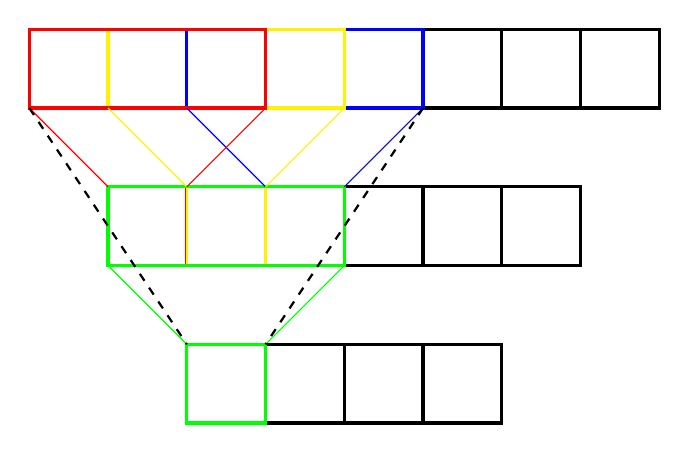
\begin{tikzpicture}[
neuron/.style={circle, draw=black, very thick, minimum size=1cm, transform shape},
dot/.style={circle, draw=black, fill=black, minimum size=0.1cm, inner sep=0pt, transform shape},
note/.style={circle, draw=black, minimum size=0pt, inner sep=0pt, transform shape},
]
%Layer 1
\draw[black, very thick] (0,  0) rectangle (1, -1);
\draw[black, very thick] (1,  0) rectangle (2, -1);
\draw[black, very thick] (2,  0) rectangle (3, -1);
\draw[black, very thick] (3,  0) rectangle (4, -1);
\draw[black, very thick] (4,  0) rectangle (5, -1);
\draw[black, very thick] (5,  0) rectangle (6, -1);
\draw[black, very thick] (6,  0) rectangle (7, -1);
\draw[black, very thick] (7,  0) rectangle (8, -1);

%Filter boxes layer 1
\draw[blue, very thick] (2,  0) rectangle (5, -1);
\draw[yellow, very thick] (1, 0) rectangle (4, -1);
\draw[red, very thick] (0, 0) rectangle (3, -1);

%Layer 2
\draw[red, very thick] (1, -2) rectangle (2, -3);
\draw[blue, very thick] (3, -2) rectangle (4, -3);
\draw[yellow, thick] (2, -2) rectangle (3, -3);
\draw[black, very thick] (4, -2) rectangle (5, -3);
\draw[black, very thick] (5, -2) rectangle (6, -3);
\draw[black, very thick] (6, -2) rectangle (7, -3);

%Filter box layer 2
\draw[green, very thick] (1, -2) rectangle (4, -3);

%Layer 3
\draw[black, very thick] (3, -4) rectangle (4, -5);
\draw[black, very thick] (4, -4) rectangle (5, -5);
\draw[black, very thick] (5, -4) rectangle (6, -5);
\draw[green, very thick] (2, -4) rectangle (3, -5);

%Connections layer 1 -- layer 2
\draw[blue] (2, -1) -- (3, -2);
\draw[blue] (5, -1) -- (4, -2);
\draw[yellow] (1, -1) -- (2, -2);
\draw[yellow] (4, -1) -- (3, -2);
\draw[red] (0, -1) -- (1, -2);
\draw[red] (3, -1) -- (2, -2);

%Connections layer 2 -- layer 3
\draw[green] (1, -3) -- (2, -4);
\draw[green] (4, -3) -- (3, -4);

%Receptive field connections
\draw[black, dashed, thick] (0, -1) -- (2, -4);
\draw[black, dashed, thick] (5, -1) -- (3, -4);
\end{tikzpicture}
\caption[Receptive field]{Three stacked convolution layers. Although all layers have a kernel size of $3$, the final layer is influenced by $5$ of the input values. Therefore the receptive field of the final layer is $5$. \textcolor{red}{Maybe change the colors and some presentation of this graphic. I don't like how it looks.}}\label{fig:receptive_field}
\end{figure}

\subsubsection{Pooling Layers}\label{sec:pooling_layers}
\textcolor{blue}{Explain what max pooling does and why it is useful, even when it is counter intuitive.}
Pooling layers are another special kind of layers, often used to increase performance of \gls{cnns}. Though there are many variations of the specific implementation, the core concept is grouping multiple activations of a single feature map into one activation. The most common pooling layer is the maximum pooling layer, as it puts greater emphasis on strong activations. \cite{max_pooling_invention} It works by grouping a certain number of input activations of the previous layer and assigning this group the maximum values of all the grouped neurons. (see \autoref{fig:max_pooling})\\
Though it does seems counter intuitive, that throwing away information helps the networks performance, the reasons are manifold. First of all pooling in general downsamples the data\footnote{There have been studies suggesting, that pooling works better than simply sub sampling the data. \cite{pooling_vs_subsampling}}. The lower number of datapoints results in fewer calculations per forward pass, fewer trainable parameters being used and thus less overfitting. Secondly, maximum pooling increases the impact of strong activations. These strong activations usually come from the parts of the data that resonate strongly with a convolution filter. If this resonance only applies for a small region in the data, there will only be few values on the feature map, that correspond to this resonance. Therefore pooling (in general) leads to greater spatial invariance. The downside of pooling is the loss of positional information. As a rule of thumb, pooling is useful for a decision ''is a feature present'', but falls short if the question ''where in the data is the feature present'' is also relevant.\\
Due to its improvement in spatial invariance, pooling also leads to the next layer having a greater receptive field.\medskip\\
All the actions described above act only on a single feature map, channel by channel. A similar approach can however also be taken for the channels themselves. Such a procedure is called \emph{dimensional reduction} and usually done through a convolution layer with a kernel size of $1$. This way, all channels are being connected through a weighted sum, where the weights are learned.\cite{dim_red_invention} Additionally a activation function can be used to introduce non-linear  combinations of the channels. In this way, dimensional reduction can not only be seen as a reduction in learnable parameters, but also as means to combine features of different channels. \cite{dim_red_interpretation} As the different feature maps are added together, this operation combines low level features into higher level ones.\\
The number of outgoing channels is given by the number of filters used in the convolution layer with kernel size $1$.
\begin{figure}
\centering
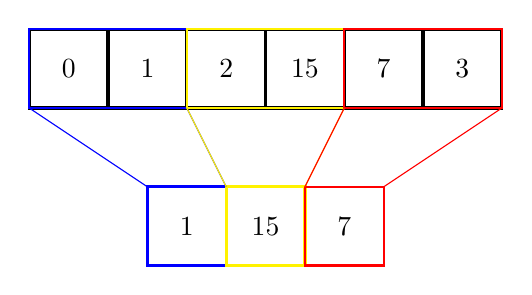
\begin{tikzpicture}[
neuron/.style={circle, draw=black, very thick, minimum size=1cm, transform shape},
dot/.style={circle, draw=black, fill=black, minimum size=0.1cm, inner sep=0pt, transform shape},
note/.style={circle, draw=black, minimum size=0pt, inner sep=0pt, transform shape},
]
%Input
\draw[black, very thick] (0,  0) rectangle (1, -1) node[pos=0.5] {0};
\draw[black, very thick] (1,  0) rectangle (2, -1) node[pos=0.5] {1};
\draw[black, very thick] (2,  0) rectangle (3, -1) node[pos=0.5] {2};
\draw[black, very thick] (3,  0) rectangle (4, -1) node[pos=0.5] {15};
\draw[black, very thick] (4,  0) rectangle (5, -1) node[pos=0.5] {7};
\draw[black, very thick] (5,  0) rectangle (6, -1) node[pos=0.5] {3};

%Filter boxes layer 1
\draw[blue, thick] (0,  0) rectangle (2, -1);
\draw[yellow, thick] (2, 0) rectangle (4, -1);
\draw[red, thick] (4, 0) rectangle (6, -1);

%Layer 2
\draw[blue, very thick] (1.5, -2) rectangle (2.5, -3) node[pos=0.5, black] {1};
\draw[yellow, very thick] (2.5, -2) rectangle (3.5, -3) node[pos=0.5, black] {15};
\draw[red, thick] (3.5, -2) rectangle (4.5, -3) node[pos=0.5, black] {7};

%Connections layer 1 -- layer 2
\draw[blue] (0, -1) -- (1.5, -2);
\draw[blue] (2, -1) -- (2.5, -2);
\draw[yellow] (2, -1) -- (2.5, -2);
\draw[yellow] (4, -1) -- (3.5, -2);
\draw[red] (4, -1) -- (3.5, -2);
\draw[red] (6, -1) -- (4.5, -2);
\end{tikzpicture}
\caption[Max Pooling layer]{An example of a Max pooling layer. It groups together two entries of its input and returns the maximum, thus halving the number of samples per feature map. This process is applied for all channels.}\label{fig:max_pooling}
\end{figure}

\subsubsection{Inception Module}\label{sec:inception_module}
\textcolor{blue}{Explain what it is, how it works. (cite google paper) ONLY IF IT IS REALLY USED IN THE FINAL ARCHITECTURE!}\\
Networks consisting of stacked convolution layers as introduced in \autoref{sec:convolution_layer} have had great success in image classification. \cite{deep_learning_book, alex_net, ILSVRC15} As the field of computer vision is one of the most prominent in machine learning and shows great advances, we use networks successfully applied there as a guideline for new architectures. Accordingly the module showcased in this section was developed for image classification and introduced in \cite{inception_module}.\\
The advantages of convolution layers over classical dense layers are manifold and discussed in further detail in \autoref{sec:convolution_layer}. One of the key advantages however is the comparatively low number of trainable parameters, as the connections are a lot more sparse. The number of these trainable parameters however is still quite large and limits the depth of a Deep-\gls{cnn}. This becomes especially obvious, when one scales the number of filters used in the convolution layers, throughout the network. If the number of filters of two consecutive convolution layers is scaled by a factor $c$, the number of trainable parameters increases by a factor of $c^2$. Scaling the number of filters is one way to increase the capacity of a network and reduce underfitting. \cite{inception_module} Another way to increase the capactity is to scale the convolution-kernel size. \textcolor{red}{Need to talk about over- and underfitting, model capacity and training data differences in a section before this one! (Probably best after the backprop section)} Larger kernels furthermore provide the capabiltiy to detect larger features within a certain part of the image. If they are too large however, the filter might be close to zero for a lot of the learnable parameters, which in turn wastes a lot of computational resources. In this situation an approach that utilizes sparse matrices or tensors would be quite beneficial, if the computational infrastructure supports it efficiently. The advantage gained by the lowered number of computations is however mostly outweight by the computational overhead created. Therefore sparse matrix operations are not feasible at the moment. \cite{inception_module}\\
A workaround for this problem is grouping multiple sparse operations together into matrices that are mostly sparse but contain dense submatrices. The matrix-operations can than be performed efficiently on the sparse matrices, by utilizing the efficient dense operations on the dense submatrices. This is the approach, the inception modules tries to take. They build a single module, that can be viewed as a layer from the outside. It contains multiple small convolution layers, that build up a larger, sparse filter. Using this new architecture, the GoogLeNet won the 2014 \gls{ilsvrc}\footnote{The \gls{ilsvrc} is a yearly competition for computer vision algorithms. It is widely used as a benchmark to judge how well a network (or any other computer vision software) does. It is always the same set of images, where each image belongs to one of about 1000 classes. The top 5 error rate is the relative number of times, the algorithm in use did not return the correct category within its top 5 choices.} image recognition competition in the category ''image classification and localization'', setting a new record for the top 5 error rate, thus proving the effectiveness of the new module. \cite{inception_module, ILSVRC15}\\
As the original work was used to handle 2 dimensional images and thus used 2D-convolutions, the module had to be slightly adjusted to fit the 1 dimensional requirements of the time series data in this work. This was a simple task however, as the difference between the two is simply the shape of the kernel and the way it is moved across the data. With Keras, there are predefined functions to handle 1D and 2D convolutions. The downside of converting the 2 dimensional inception module to a 1 dimensional one however is, that many of the incremental improvements to the module are not applicable, as they rely heavily on the 2D-structure. \cite{inception_v2_v3, inception_v4}\medskip\\
The following paragraphs will describe the module used in this work in greater detail.\\
The module consists of 4 independent towers, each consisting of different layers. The full module is depicted in \autoref{fig:inception_module}.\\
The module consists of three parallel convolution layers, i.e. each of the three layers share the same input. The difference between them is the kernel size. The convolution layers with a larger kernel a preceded by a convolution layer with $16$ filters and a kernel size of $1$. The purpose of this step is to reduce the number of channels used and is called dimensional reduction. This leads to a fixed input size for the larger kernels, regardless of the depth of the input. 
In the original architecture filters of size $1\times1$, $3\times3$ and $5\times5$ were used. Translating them directly to 1 dimensional equivalents, the module should use kernel sizes of $1$, $3$ and $5$. However we empirically found, that the smallest kernel sizes $1$, $2$ and $3$ performed best. \textcolor{red}{(Did I ever try 1,3,5? If not do so!)}\\
Finally a pooling layer as introduced in \autoref{sec:pooling_layers} is added as a fourth path. The reasoning behind this step is, that pooling layers have shown great improvements in traditional \gls{cnns} and thus the network should be provided with the option to choose this route as well. For this layer the dimensional reduction takes place only after the pooling procedure.\\
The output of each of these paths is than concatenated along the last axis of the tensor, i.e. along the different channels. For this reason all input to each of the layers is padded with zeros in such a way, that the shape (except for the channels) does not change.
\begin{figure}
\centering
\begin{tikzpicture}[
neuron/.style={circle, draw=black, very thick, minimum size=1.0cm},
dot/.style={circle, draw=black, fill=black, minimum size=0.1cm, inner sep=0pt},
VLineVertex/.style={circle, draw=black, minimum size=0cm, inner sep=0pt},
layer/.style={rectangle, draw=black, very thick, minimum height=1cm, minimum width=3cm},
concat/.style={rectangle, draw=black, very thick, minimum height=1cm, minimum width=6.5cm}
]

%Nodes
\node[layer] (input) {input};
\node (midpoint) [below=1cm of input] {};
\node[layer] (l_2_dim_red) [left=0.25cm of midpoint] {Conv1D$\lr{16, 1}$};
\node[layer] (l_2_filter) [below=0.5cm of l_2_dim_red] {Conv1D$\lr{64, 2}$};
\node[layer] (l_1) [left=0.5cm of l_2_dim_red] {Conv1D$\lr{96,1}$};
\node[layer] (r_2_dim_red) [right=0.25 of midpoint] {Conv1D$\lr{16, 1}$};
\node[layer] (r_2_filter) [below=0.5cm of r_2_dim_red] {Conv1D$\lr{32, 3}$};
\node[layer] (r_1_pool) [right=0.5cm of r_2_dim_red] {MaxPooling$\lr{4}$};
\node[layer] (r_1_dim_red) [below=0.5cm of r_1_pool] {Conv1D$\lr{32, 1}$};
\node[concat] (concat) [below=2.5cm of midpoint] {Concatenate Channels};

%Connections
\draw (input.south) -- (l_1.north);
\draw (input.south) -- (l_2_dim_red.north);
\draw (input.south) -- (r_2_dim_red.north);
\draw (input.south) -- (r_1_pool.north);

\draw (l_2_dim_red.south) -- (l_2_filter.north);
\draw (r_2_dim_red.south) -- (r_2_filter.north);
\draw (r_1_pool.south) -- (r_1_dim_red.north);

\draw (l_1.south) -- (concat.west);
\draw (l_2_filter.south) -- (concat.north);
\draw (r_2_filter.south) -- (concat.north);
\draw (r_1_dim_red.south) -- (concat.east);
\end{tikzpicture}
\caption[Inception module]{Shown are the contents and connections of the inception module as used in this work. \textcolor{red}{(If the filter numbers and values change for the final architecture, change them here too.)} The layer Conv1D$\lr{x,y}$ is a 1 dimensional convolution layer with $x$ filters and a kernel size of $y$. Most of the convolution layers with a kernel size of $1$ are used for dimensional reduction. The only exception is the leftmost one, that consists of $96$ filters. The different filter sizes correspond to the ability of detecting features at different scales. The pooling layer is a 1 dimensional pooling layer, that only passes on the maximum value in a bin of size 4. The final layer concatenates the channels of the different towers. This also means, that each tower needs to have the same output-shape, excluding the channels. For this reason all inputs are automatically padded with zeros in such a way, that the output-shapes are correct.}\label{fig:inception_module}
\end{figure}

\subsubsection{Temporal Convolutional Networks}
\textcolor{blue}{Explain what they are, what their advantages are and list works that utilized them.}
Temporal convolutional networks (\gls{tcn}), as used in this work, were proposed by \cite{tcn_paper}. Their research suggests that this specialized \gls{cnn}-architecture outperforms \gls{rnns}, which were previously the norm for analyzing and processing sequence data.\\
A \gls{tcn} basically consists of multiple stacked convolution layers, that are slightly adapted in two different ways. For once, the filters are diluted, meaning, that the weighted sum of the convolution is not taken over successive input points. Instead the weighted sum uses points, skipping a set number of inputs in between. Secondly the connections are causal. This means, that output $y_i$ of the filter depends at most only on points $x_i, \dotsc,x_1$. Finally the input of each such layer is padded with zeros such, that the output matches the size of the input. (see (a) of \autoref{fig:tcn})\\
The advantage of the dilated convolution layers is, that the receptive field of the network grows exponentially with the depth, whereas without the dilution this growth is only linear. \textcolor{red}{[Citation]} The goal of the \gls{tcn} is to have a receptive field, that spans the entire input length. This still requires a decently deep network for inputs of considerable length. To combat the problem of the vanishing gradient, residual connections are also introduced. The dimensional reduction layer that is part of the residual connection is simply used to adjust the number of channels to be able to add the input and the output of the residual block together. The full structure of the residual block is shown in (b) of \autoref{fig:tcn}. The only adaption to the implementation that this work makes is the the replacement of the WeightNorm layer with a traditional BatchNormalization layer, as it is described in \autoref{sec:batch_norm}. This is done for convenience, as there is a pre-implemented version of batch normalization in the software library used. This replacement is valid, as weight normalization is described by the authors to be largely a fast approximation to full batch normalization. \cite{weigth_norm_invention}
\begin{figure}
\centering
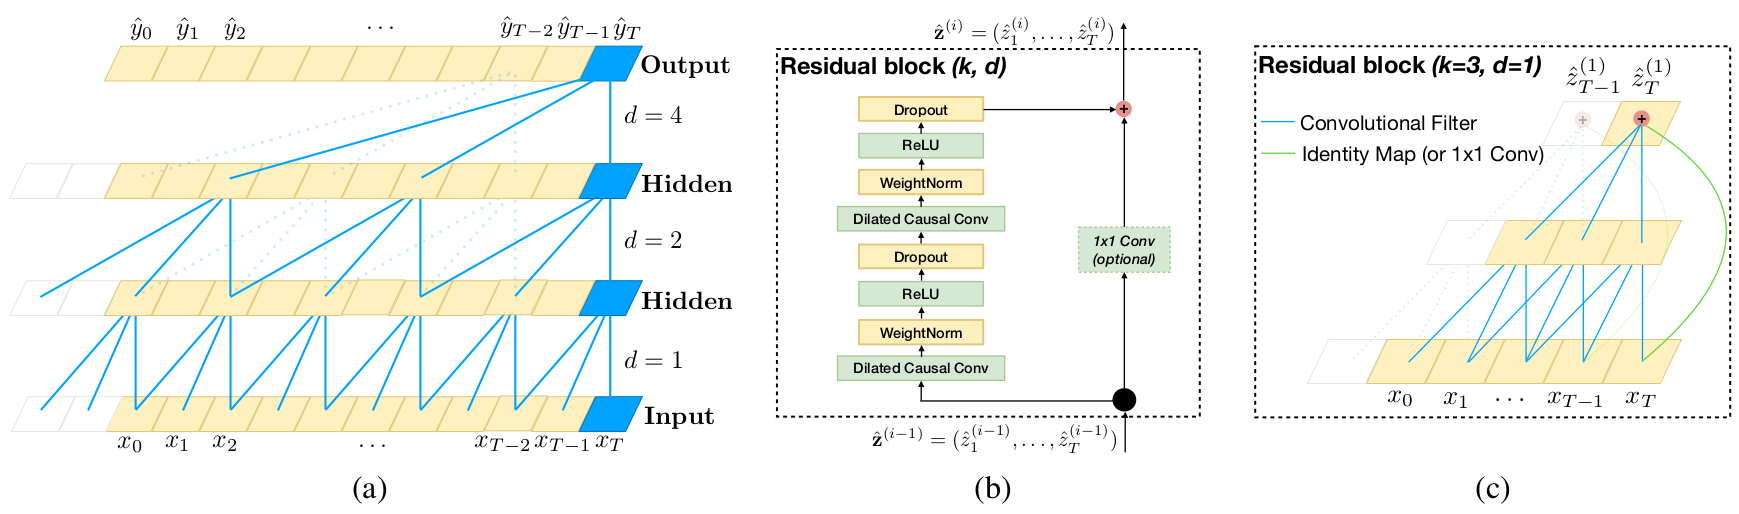
\includegraphics[width=\textwidth]{TCN.png}
\caption[TCN structure]{Architectural elements in a \gls{tcn}. Graphic taken from \cite{tcn_paper}. (a) Exponential increase of the receptive field in diluted convolution layers. Here the dilution factor $d$ scales as $2^i$ and the kernel size $k$ is set to $3$. The causal structure propagates through the layers, as no output is connected to an earlier input. (b) Multiple different layers are utilized for an entire module of the \gls{tcn}. Also a residual connection is used, to help earlier levels learn. Multiple of these units are stacked to form a \gls{tcn}. (c) An example of how the residual block from (b) could look like.}\label{fig:tcn}
\end{figure}


\subsection{Regularization}\label{sec:regularization}
As \cite{deep_learning_book} put it: ''Regularization is any modification we make to a learning algorithm that is intended to reduce its generalization error but not its training error.''. There are many ways, like reducing the number of trainable parameters or adjusting the loss function to prefer specific weights, to achieve this goal. This section however will only introduce two specialized methods, that are introduced as a layer into the network.

\subsubsection{Batch Normalization Layer}\label{sec:batch_norm}
\textcolor{blue}{Explain how batch normalization works and why it is useful. (cite according paper)}
Batch normalization was introduced in \cite{batch_normalization_invention} and is used to normalize the inputs of each layer. This helps the network learn faster and generalize more easily.\\
The normalization tries to fix the distribution of the inputs between different samples, as the layers would need to adapt their weights otherwise for different input distributions. Specifically the goal is to transform the data in a way, that the mean is $0$ and the variance is $1$. Normalizing data in such a way is in principle not problematic and a standard procedure only for the input layer. \textcolor{red}{[Citation]} The problem of normalizing the input of each individual layer is the backporpagation step, as it can lead to exploding biases. \cite{batch_normalization_invention}\\
To solve this issue, gradients of the normalization with respect to multiple inputs need to be computed. Batch normalization uses the samples of each mini-batch to compute the mean, variance and gradients. To reduce computational cost, the normalization is computed only over one dimension of the input. In this work, the mean and variance will be calculated for every channel and thus applied to each channel individually. Finally a linear transformation
\begin{equation}
y_i = \gamma \hat{x}_i + \beta
\end{equation}
is applied to the normalized data
\begin{equation}
\hat{x}_i = \frac{x_i - \mu_B}{\sqrt{{\sigma_B}^2 + \varepsilon}}.
\end{equation}
Here $x_i$ is the $i$-th sample of the mini-batch, $\mu_B$ is the mean and ${\sigma_B}^2$ is the variance of the activations calculated over the mini-batch. The factors $\beta$ and $\gamma$ are learned parameters and $\epsilon$ is a constant added for numerical stability.\\
The linear transformation is applied so that the batch normalization layer can learn to be the identity transformation. Otherwise the normalization could loose the ability to represent some function it previously could have represented.\medskip\\
The implementation in Keras differs from this approach in the sense, that the mean $\mu_B$ and variance ${\sigma_B}^2$ are only calculated for each individual batch during training. When the network is used to evaluate some data, it will use a fixed mean and variance, that was approximated over all batches during training. They call this the moving average $\mu_\text{mov}$ and moving variance $\sigma_\text{mov}^2$ respectively and adjust them after every batch by
\begin{align}
{\mu'}_\text{mov} & = m\cdot\mu_\text{mov} + \lr{1-m}\mu_B\nonumber\\
{{\sigma'}_\text{mov}}^2 & = m\cdot{\sigma_\text{mov}}^2 + \lr{1-m}{\sigma_B}^2,
\end{align}
where $m$ is the momentum used and usually set to a high value around $0.99$. Using this has the advantage, that only a finite number of samples have a non negligible effect on the mean- and variance value used during inference. Therefore drifts in the input distribution, which might occur during training, can be counteracted.

\subsubsection{Dropout Layer}
\textcolor{blue}{Explain what a dropout layer is, what it does, why it is useful.}\\
Dropout layers were introduced in 2014 by \cite{dropout_invention} and showed great improvements to lowering the generalization error. It works by dropping a random percentage of neurons from the network during training. Though this approach sounds counter intuitive, it has multiple benefits.\\
One viewpoint is using the dropout layer as a noise source for the network. By dropping some activations during training, the network can't be too strongly dependent on a single connection and has to learn multiple ways of detecting some feature. Therefore the network becomes less sensitive to small alterations of the input. Furthermore the dropout layer can be used as a first layer in a network and act as data augmentation, where it introduces further noise to the data, as  the same sample may experience different dropped connections. Therefore the effective number of samples the network sees during training is enlarged.\\
Another viewpoint is, that training a network with dropout layers does not only tryout the full architecture, but also all sub-networks, that can be created from the full architecture by dropping some connections. The number of sub-networks grows exponentially with the number of dropout layers. This viewpoint is the main selling point promoted by \cite{deep_learning_book} and \cite{dropout_invention}, as it allows to efficiently sample many networks and combine them.\\
During the evaluation process, the original paper \cite{dropout_invention} suggests reweighing the weights by the dropout probability, to get an averaging effect. This step is however not done in the software library Keras used in this work. \textcolor{red}{[Citation]}
